%!TEX root = main.tex
%%%%%%%%%%%%%%%%%%%%%%%%%%%%%%%%%%%%%%%%%%%%%%%%%%%%%%%%%%%%%%%%%%%%%%%%%%%%%%%%

\section{Methodology}

\label{sec:sysmodel}

In this section we discuss the two approaches we use to evaluate the observed adaptation from the experimental data set.
This first approach is based on regression and uses previously observed video sessions to create an estimation on how much non-redundant traffic relates to a specific average playback quality.
This has the advantage of being fast, scalable and not computational expensive. 
Furthermore, as it is based on actual observed data, it captures the dynamics of the deployed system.
We use this estimation then to calculate the maximum achievable average quality level based on the total amount of downloaded Bytes in a playback session.
The second approach is based on a mixed integer linear program (MILP) formulation. 
For this optimization problem we take the actual video segment sizes, the observed bandwidth and cumulative stallings times from the experimental data set as an input.
This gives us the optimal adaptation considering the stallings times.
In a second step, we remove the cumulative stalling times and force the optimization problem to instantly play the video.

%!TEX root = main.tex
%%%%%%%%%%%%%%%%%%%%%%%%%%%%%%%%%%%%%%%%%%%%%%%%%%%%%%%%%%%%%%%%%%%%%%%%%%%%%%%%

\subsection{Heuristic Approach}

The heuristic approach uses isotonic regression \cite{barlow1972statistical} to deduce a video-dependent relationship between the data shown to the user and the resulting average quality level based on previously recorded playback sessions.
This gives an estimate of how much non-redundant data is necessary to reach a certain quality level.
Furthermore, it allows us to estimate the difference in term of average quality between two different amounts of data.
The advantage of the approach is that it captures the dynamics of the overall system as it is based on actual observations.

\begin{figure}[t]
\centering
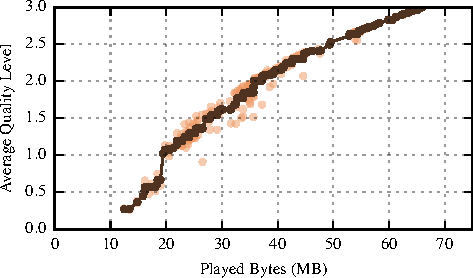
\includegraphics[width=0.9\linewidth]{figs/32_vbLLqaa9ksw.pdf}%
\caption{Isotonic regression result showing the relationship between Bytes shown to the user and resulting average playback quality for video vbLLqaa9ksw. 336 video views are used in the regression.}
\label{fig:heuristic}%
\end{figure}

Figure \ref{fig:heuristic} illustrates the resulting relationship denoted as function $\phi$ for one of the videos in the data-set.
The axis to the right gives the amount of Bytes shown to the user.
The axis to the left gives the resulting average playback quality.
Each (brown) dot represents one playback session.
The connected (black) dots are the isotonic regression result.

Multiple observations can be made from the figure. 
First, a specific amount of played bytes can result in different average quality levels at the end. 
This is due to the combinatorial problem which arises due to the different quality levels and bit-rate variations inside a quality level.
Second, there is a jump at \unit[20]{MBytes} from 0.7 to 1.1 average quality level.
Third, there are outliers, e.g. at \unit[27]{MBytes}, where significant more data does not increase the average quality level.

Based on $\phi$ we determine the loss in average quality level due to the redundant traffic as:

\begin{equation}
\phi(B_T) - \phi(B)
\end{equation}

%!TEX root = main.tex
%%%%%%%%%%%%%%%%%%%%%%%%%%%%%%%%%%%%%%%%%%%%%%%%%%%%%%%%%%%%%%%%%%%%%%%%%%%%%%%%
\subsection{Optimal Adaptation}
\label{optadapt}

In order to determine how much potential there is for optimization, we formulate a MILP for this problem. 
The solution to the MILP will return an optimal adaptation with respect to available bandwidth, video segment sizes, and cumulative stalling times.

A given video is available in $r$ resolutions and consists of $n$ segments, i.e. each segment can be played in exactly one resolution. Furthermore, each segment $i$ that is played in resolution $j$ has a size $S_{ij}$. We assume that all segments have the same duration $\tau$ and are downloaded in order. The total data that has been downloaded at the point in time $t$ is $V(t)$. Before a segment can be played, it has to be downloaded. This means there is a deadline $D_i$ until which the segment must be downloaded if no stalling may occur. Since there is an initial delay $T_0$ before the first segment can be played, according to \cite{hossfeld2015identifying} the deadline is

\begin{equation}
D_i = T_0 + i\cdot \tau.
\end{equation}

The goal is to optimize the downloading process so that the video may be played with the highest average resolution. This leads us to a MILP which is a special case of \textit{Optimization Problem 2} from \cite{hossfeld2015identifying}.

\begin{align*}
& \text{maximize} & \sum_{i = 1}^{n} \sum_{j = 1}^{r_{\text{max}}} j x_{ij} &\\
& \text{subject to} & &&\\
&& x_{ij} &\in \{0,1\} &\\
&& \sum_{j = 1}^{r_{\text{max}}} x_{ij} &= 1, &\forall i&=1,\ldots,n \\
&& \phantom{\text{.}} \sum_{i=1}^{k} \sum_{j = 1}^{r_{\text{max}}} S_{ij} x_{ij} &\leq V(D_k), &\forall k&=1,\ldots,n \text{.} \\
\end{align*}

Above problem is the Multiple-Choice Nested Knapsack Problem which is NP-hard. However, there exist polynomial time algorithms that return an approximation for the optimal solution that is sufficiently good for most practical purposes. The MILP was implemented in Gurobi \footnote{http://www.gurobi.com/} with MATLAB.

%!TEX root = main.tex
%%%%%%%%%%%%%%%%%%%%%%%%%%%%%%%%%%%%%%%%%%%%%%%%%%%%%%%%%%%%%%%%%%%%%%%%%%%%%%%%

\subsection{Data Sets}

In total, we acquired four data sets that are used in the evaluation. Two of those are data sets from \cite{sieber16sacrificing}. The other two were created by implementing above optimization problem in the Gurobi Optimizer\footnote{http://www.gurobi.com/}.

First, we have the initial observations which shall serve as the \textit{baseline} in the following analysis. These measurements were originally recorded in \cite{sieber16sacrificing} where the measurement methodology and measurement set-up is described in great detail: $35$ videos $\times 27$ bandwidth values $\times 15$ replications. Four quality level representations were observed: $144p, 240p, 360p, 480p$. In the following, we refer to these video quality levels as $0,1,2,3$. Please notice that stalling events did occur in $56\%$ of these runs.

Based on this data set, we used the heuristic approach described in \ref{sec:heu} to estimated the average resolution that is reachable if there was no redundant traffic, i.e. when no video segment is downloaded multiple times. Notice that it was assumed that the same amount of stalling would occur.

As a new contribution, we use the optimization problem, described in Section \ref{optadapt} to exactly calculate the highest mean resolution that was optimally obtainable. As a second step, the number of switches is minimized as first proposed in \cite{miller2013optimal}. For both steps, we limited the execution time of the Gurobi Optimizer to $\SI{1}{\second}$ in order to process the complete data in a timely manner. Increasing the execution will most likely lead to slightly better values than presented in the following. For this two-step approach, we consider the same video files, the same duration of the viewing session and the same average network throughput as was used in the baseline scenario to make it comparable. However, instead of having stalling events interrupt the replaying process, we added an initial delay to the the replaying process. The duration of this delay is equal to the sum of the observed stalling events. This leads to the same duration of the viewing session and the same replay time and the same amount of data that was totally downloaded. In the following, we refer to this scenario as \textit{opt (prebuffering)}.

Lastly, we present a data set that is obtained in the same fashion as \textit{opt (prebuffering)} with one mayor difference: the video started replaying as soon as the first segment was fully downloaded. To achieve this, we considered the exact same network throughput as in the baseline scenario, while having a shorter session duration since the stalling times are omitted. This means that the amount of data that is downloaded in this case is lower than in the baseline scenario. In the following, we refer to this scenario as \textit{opt (instant play)}.

